\chapter{Konzept}
% idee vorstellen 
%s\subsubsection*{Stichworte}
%\begin{itemize}
%\item Übersicht von Konzept mit Graphik
%\item 3 Bereiche aufzeigen: EEROS, Gazebo, RQt \& rviz
%\item Schnittstellen zu einander
%\item Verweis zu Mäsis Arbeit
%\item URDF, SDF vorstellen und erklären, hier??? oder in Motor
%\end{itemize}
%TODO erwähnen systemen -> ist eine mechatronisches system gemein aus Aktor,...  -> roboter

Eine Skizze des Konzeptes ist in der Abbildung \ref{Ab:konzept}
zu sehen.
Die zwei Hauptkomponenten sind \textit{EEROS} und \textit{ROS}.
\textit{EEROS} übernimmt in diesem Szenario die Aufgabe des Reglers.
Und \textit{ROS} die Aufgaben der Simulation und der Visualisierung.

\begin{figure}[ht!]
	\centering
	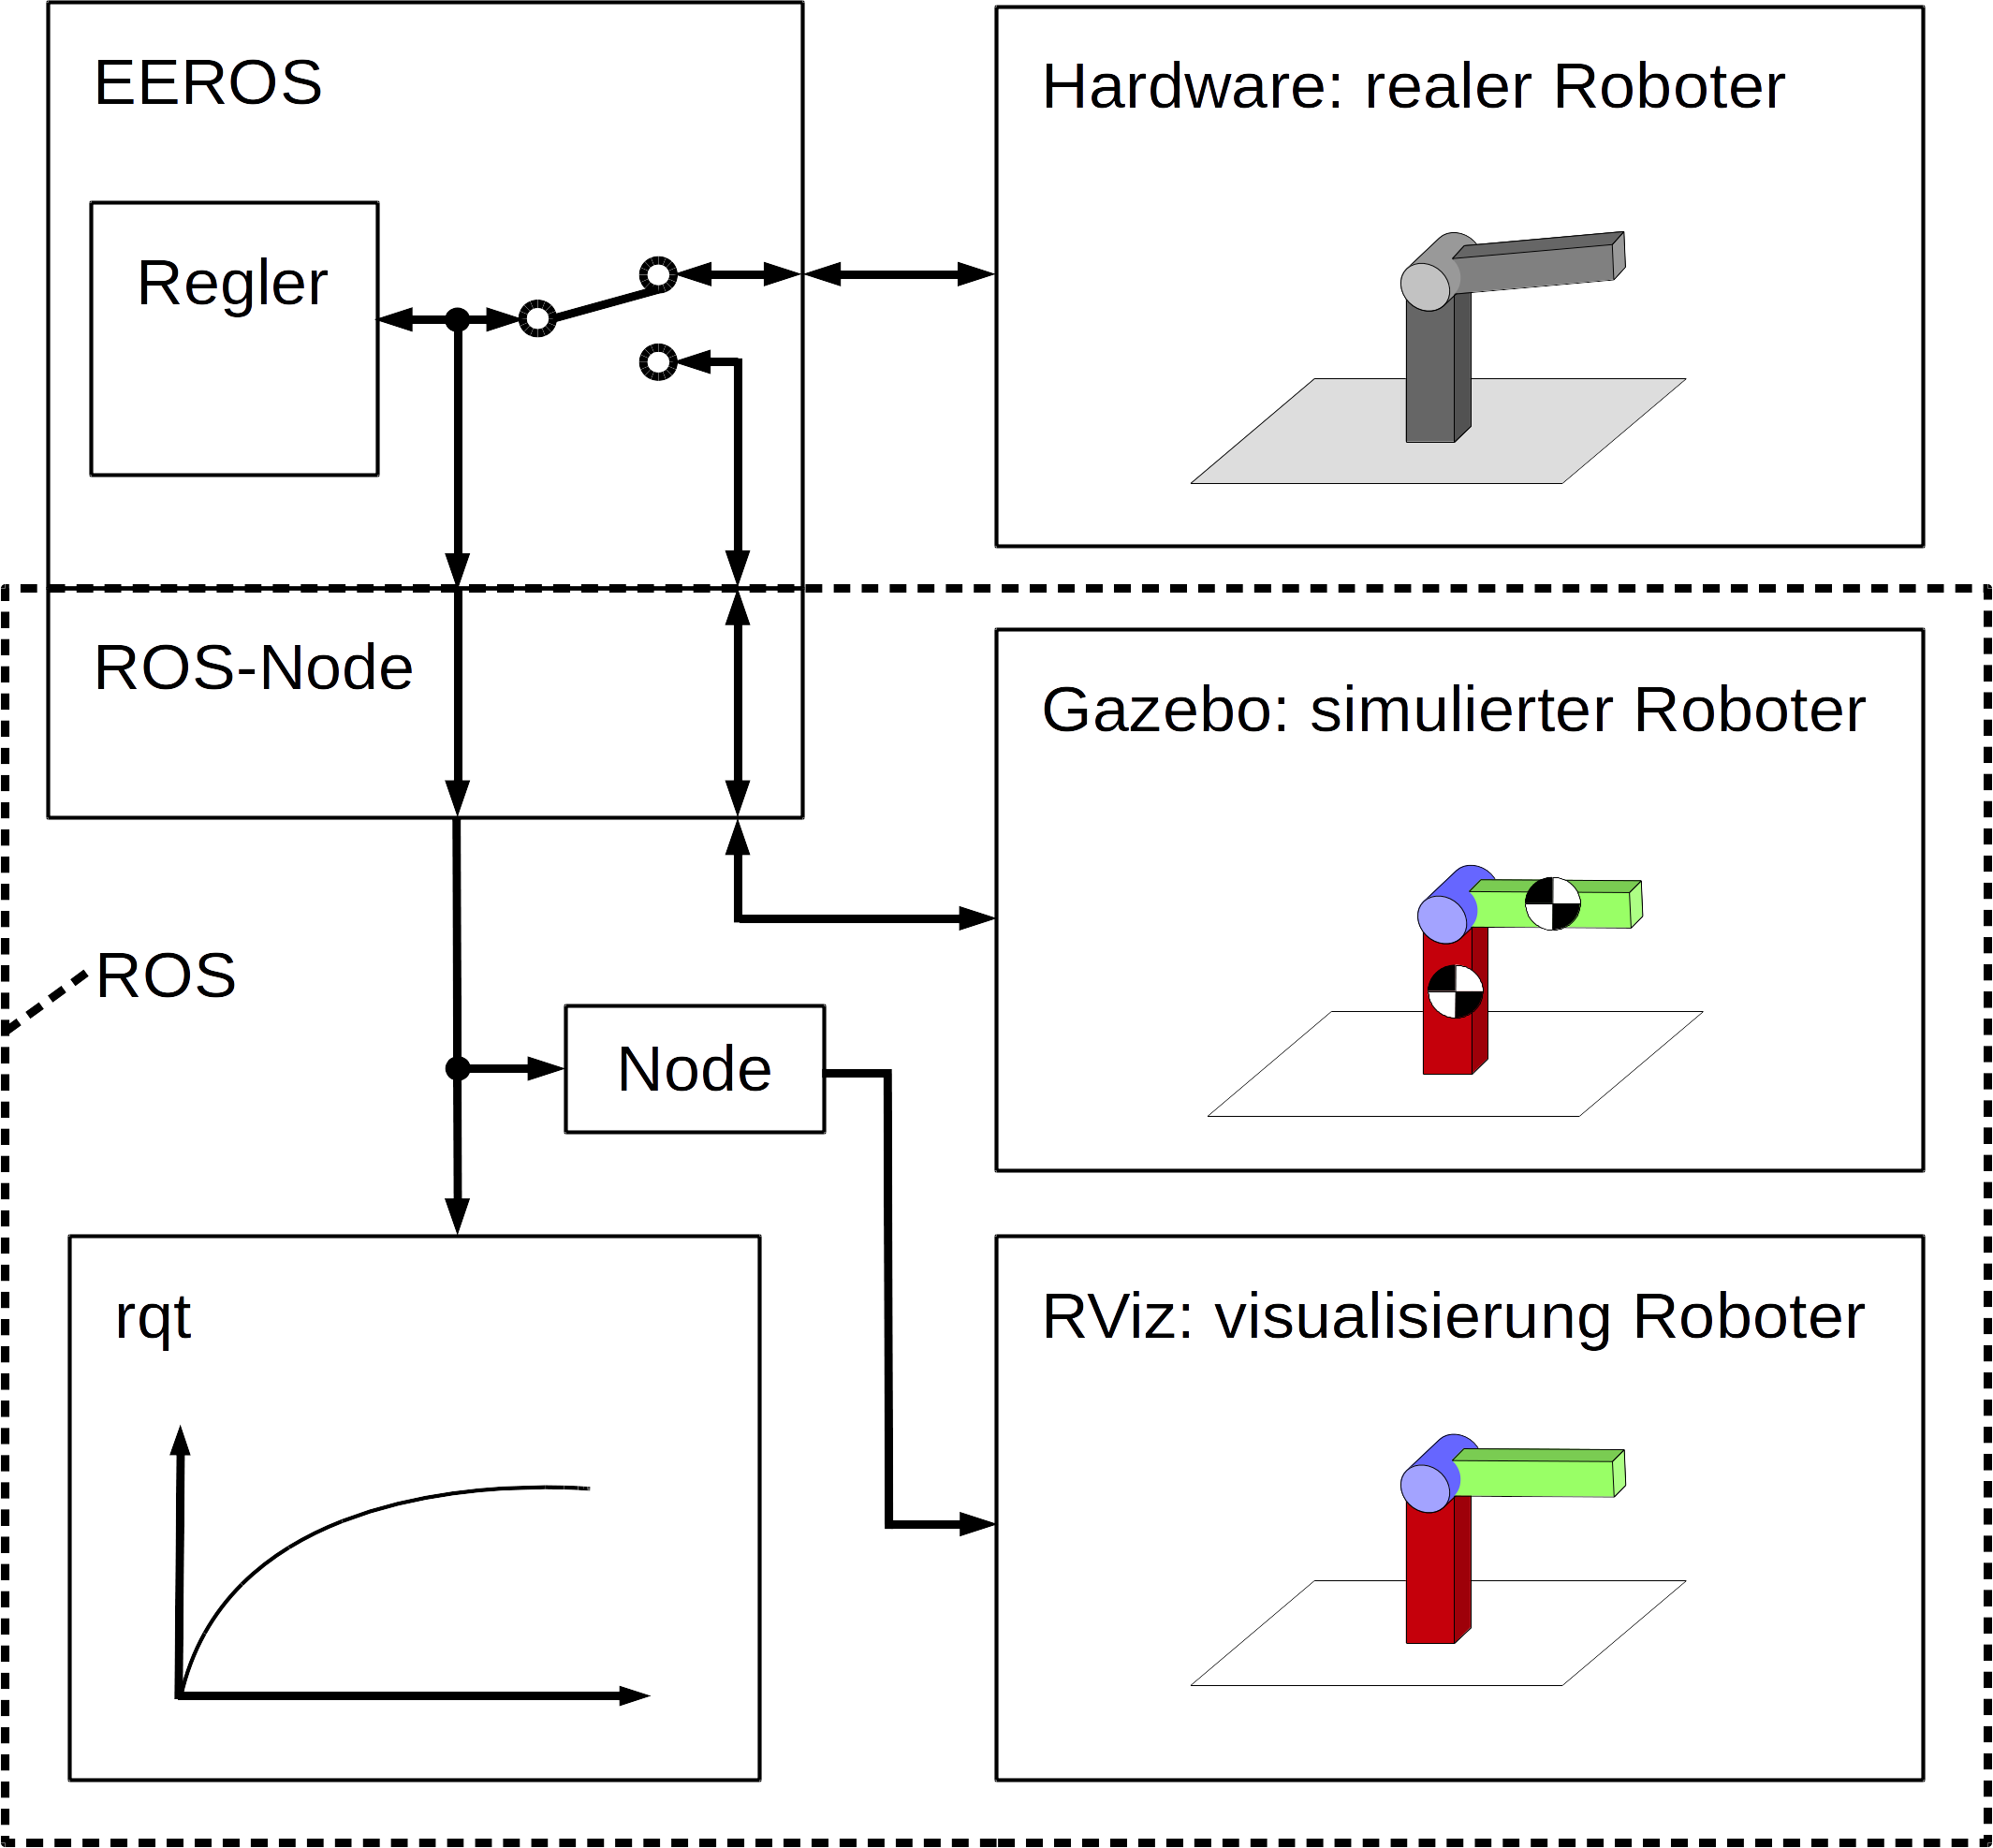
\includegraphics[width=14.5cm]{images/Konzept.png}
	\caption{Konzept}
	\label{Ab:konzept}
\end{figure}

Damit \textit{EEROS} mit \textit{ROS}"=Komponenten kommunizieren kann, wurde ein \textit{ROS}"=Node ins \textit{EEROS} integriert.
Diese Integration wird in der Arbeit xx erklärt. %TODO ref mäsis arbeit
Somit hat \textit{EEROS} die Fähigkeit über das \textit{ROS}"=Kommunikationsprinzip \textit{Publish\,\&\,Subscribe} Daten auszutauschen.
Das Konzept sieht vor, das \textit{EEROS} wahlweise einen echten oder simulierten Roboter steuert und regelt.
%Mit dem Begriff System werden in dieser Arbeit allgemein mechatronische Systeme wie zum Beispiel ein Roboter bezeichnet.
Der Roboter in der Skizze ist aus zwei Gliedern und einem Gelenk aufgebaut.
Die Stellgrösse die von \textit{EEROS} vorgegeben wird ist das Drehmoment für das Gelenk.
Und die Regelgrösse ist die Winkelposition des Gelenks.

Die Visualisierung mit \textit{RQt} und \textit{RViz} erfolgt gleichermassen, ob ein echter oder simulierter Roboter betrieben wird.
Mit \textit{RQt} können die Grössen in Plots dargestellt werden, und der Zustand des Roboters kann mit \textit{RViz} visualisiert werden.
Da \textit{RViz} nicht direkt die Gelenkwinkel interpretieren kann, müssen diese von einem \textit{ROS}"=Knoten\footnote{siehe Kapitel \ref{chap:robot-state-publiseher}} in Koordinatensystem"=Transformationen\footnote{siehe Kapitel \ref{chap:transformationen}} umgerechnet werden.

%Zu und vom System fliessen Daten wie Stell"= und Regel"=Grössen.
%Diese Daten werden einfachheitshalber Grössen genannt.
%Aus den Grössen die vom Roboter kommen kann der Zustand vom System interpretiert werden.
%Der Zustand von einem System kann zum Beispiel die Winkel"=Position eines Motors beschreiben.

%Die Zustände und Grössen eines Systems werden visualisiert egal ob an einem realen oder ein simulierten System gearbeitet wird.

%Für die Simulation von Systemen wird \textit{Gazebo} eingesetzt.
%Die Darstellung von den System Zuständen wird mit \textit{rviz} realisiert.
%Für die Visualisierung der Grössen werden Plots eingesetzt.
%Für das erzeugen der Plots wird das \textit{RQt} Plugin multiplot eingesetzt.

%Das Konzept kann in mehrere Bereich aufgeteilt werden.
%Die Simulation des Systems, die Visualisierung des Zustandes vom System und der KontrollerEEROS.


%\begin{tikzpicture}[scale=4]
%%	\draw (0, 0) -- (14.5, 0);
%%	\draw (0, 0) -- (0, 1.5)
%%	(0,0) rectangle ++(10,2);
%	\draw[step=0.5]
%	(0,0) grid (1.4,1.4);
%	
%	\draw[->] (0,0) -- (1.5,0) node[right] {$x$};
%	\draw[->](0,0) -- (0,1.5);
%	
%	\draw
%	(1,0) arc (0:90:1cm)
%	(3mm,0pt) arc (0:30:3mm);
%	
%	\draw 
%	(0,0) -- node[below] {blaa} (1,0);
%	
%\end{tikzpicture}
%
%\begin{tikzpicture}[scale=1,node distance=5mm]
% \path
% 	(8,4) node {Eingabe}
% 	(8,3) node {$r=a$}
% 	(8,0) node {Ausgabe};
%% 	
%% \node at (4,4) (eingabe) {Eingabe};
%% \node at (4,3) (blaa) {$r=a$};
% 	
% \node (in) {Eingabe};
% \node[below=of in] (div) {$r=a$};
% 
% \path[->]
% 	(in) edge (div);
% \draw[->]
% 	(div) -- ++(1,0) |- (in);
%
%\end{tikzpicture}
%
%%\centering
%\begin{tikzpicture}[
%		scale=1,
%		%every node/.style={transform shape},
%		eeros/.style 2 args={draw, rectangle, minimum height=#1, minimum width=#2}]
%	\node (eeros) [eeros={1}{1}] {EEROS};
%	
%\end{tikzpicture}
%
%\begin{lstlisting}[language=Java]
%public class Hello {
%	public static void main(String args[]) {
%		System.out.println("hello world");
%	}
%}
%\end{lstlisting}
%
%\framebox{}

\section{Gazebo}
\label{chap:gazebo}
\textit{Gazebo} ist eine Starrkörper"=Simulationsumgebung für Mehrkörper"=Systeme.
Vom System das man simulieren möchte, muss eine System"=Beschreibung in Form von einer \textit{SDF}"=Datei erstellt werden.
\textit{Gazebo} baut dann die Simulation anhand dieser Datei auf. 
In unserem Fall wird im \textit{SDF}\footnote{siehe Kapitel \ref{chap:sdf}} das Roboter"=Modell beschrieben.

Mit Plugins kann \textit{Gazebo} mit Funktionen erweitert werden.
Dabei kann man schon fertige Plugins verwenden, oder selber eines programmieren.
Im Zusammenhang mit diesem Konzept, werden die Plugins für die Kommunikation mit dem \textit{EEROS} eingesetzt.
Ein Plugin wird für das Applizieren der Stellgrösse (Drehmoment) auf das Gelenk eingesetzt und eines für die Messung und Rückführung (publish) des Gelenkwinkels.


\section{RViz}
\label{chap:rviz}
Mit dem Visualisierungs"=Tool \textit{RViz} kann der Zustand vom Roboter visualisiert werden.
Der Zustand ist die momentane Stellung von den Gelenken des Roboters, oder einfacher ausgedrückt die Pose des Roboters.
Auch wird \textit{RViz} eingesetzt für die Visualisierung von anderen Daten wie z.B. die Sensor"=Daten einer 3D"=Kamera.

Damit \text{RViz} den Zustand vom Roboter darstellen kann, braucht es folgende Informationen:
\begin{itemize}
\item Aussehen jedes Glieds des Roboters, wie Form und Farbe 
\item laufend für jedes Glied: Position und Orientierung
\end{itemize}

Mit einer \textit{URDF}"=Datei\footnote{siehe Kapitel \ref{chap:urdf}} müssen dem \textit{RViz} die Information über das Aussehen zur Verfügung gestellt werden.
\textit{URDF} ist ein Format für die Modell"=Beschreibung eines Roboters.
In \textit{RViz} muss immer ein Koordinatensystem als fixe Referenz angegeben werden.
Normalerweise wird das Welt"=Koordinatensystem gewählt.
Um ein Körper im Raum darzustellen, braucht \textit{RViz} eine Angabe zur Position und Orientierung, relative zum Referenz"=Koordinatensystem.
Diese Angabe wird als Transformation\footnote{siehe Kapitel \ref{chap:transformationen}} bezeichnet.
\textit{RViz} erhält laufend diese Transformations"=Daten von einem \textit{ROS}"=Knoten und kann anhand von diesen, den aktuellen Zustand des Roboters visualisieren.

%Und aus den Transformations"=Daten die \textit{RViz} laufend erhält, kann es die Position und Orientierung jedes Körpers berechnen.
%Und Informationen über die Position und Orientierung jedes Körpers kann \textit{RViz} über Transformationen.
%Eine Transformationen beschreiben wie ein Koordinatensystem relative zu einem anderen steht.   

%Für die Darstellung der Körper im Raum benötigt \textit{rviz} für jeden Körper noch die Position und Orientierung von diesem im Raum.
%Deshalb müssen dem \textit{rviz} stetig Koordinaten-Daten für jeden Körper übermittelt werden. %TODO ref tf


\section{RQt}
\label{chap:rqt}
\textit{RQt} ist Framework für die GUI Entwicklung in \textit{ROS}.
Diese GUI's werden als Plugins implementiert.
Somit können mehre GUI's in einem \textit{RQt}"=Fenster verwendet werden.
Für fast jedes gängige \textit{ROS}-Command-line-Tool gibt es schon Plugins\footnote{\url{http://wiki.ros.org/rqt/Plugins}}.
Es können aber auch selbst programmierte Plugins verwendet werden. 
Für die Visualisierung von zeitabhängigen Grössen wird das \textit{RQt}"=Plugin \textit{multiplot}\footnote{\url{http://wiki.ros.org/rqt_multiplot}} eingesetzt. %TODO bild?

%gui-tool, für das plugins vorhanden sind oder selber geschrieben werden können
%hat für viele gängige ros-cli-tools ein RQt-plugin


\section{Roboter-Modell} % Roboter"=Modell
\label{chap:roboter-modell}
%TODO titel mehrdeutig mehr so was wie: Datei-formate für beschreibung von Systemen, repräsentation, abbildung, Format für repräsentation von Systemen

Die Programme \textit{Gazebo} und \textit{RViz} verwenden zwei unterschiedliche Datei"=Formate für die Modell"=Beschreibung.
Beide sind im XML"=Stil gehalten und repräsentieren kinematische Strukturen.
Diese Strukturen sind aus Gliedern (Links) und Gelenken (Joints) aufgebaut.
%Der Aufbau eines Modells wird im Kapitel xx erleutert.

\subsection{URDF-Unified Robot Description Format}
\label{chap:urdf}
Das \textit{URDF}"=Format\footnote{\url{http://wiki.ros.org/urdf}} wird standardmässig in \textit{ROS} verwendet für die Beschreibung von Robotern.
Es kann nur kinematische Strukturen abbilden die eine Baum"=Form haben.
Somit können keine geschlossenen kinematischen Ketten beschrieben werden.
Im Kapitel \ref{chap:urdf} wird beschrieben, wie ein \textit{URDF}"=Model aufgebaut werden kann.

\subsection{SDF-Simulation Description Format}
\label{chap:sdf}
Das \textit{SDF}"=Format wird bis jetzt ausschliesslich im \textit{Gazebo} verwendet.
Es kann kinematische Graph-Strukturen abbilden.
Deshalb können auch geschlossene kinematische Ketten beschrieben werden.

\subsection{Konvertierung URDF zu SDF}
\label{chap:konvertierung}
Damit für ein Roboter nicht zwei Dateien erstellt und instand gehalten werden müssen gibt es eine Lösung.
Die Lösung besteht darin die \textit{URDF}"=Datei in eine \textit{SDF}"=Datei zu konvertieren.
Die Konvertierung erfolgt im \textit{ROS}"=Node \textit{\textit{"}urdf\_spawner"} \footnote{\url{https://github.com/ros-simulation/gazebo\_ros\_demos/blob/kinetic-devel/rrbot\_gazebo/launch/rrbot\_world.launch}} zur Laufzeit, wenn das Roboter"=Modell in die Simulations"=Umgebung von \textit{Gazebo} geladen wird.
Das \textit{URDF}"=Format ist jedoch nicht so mächtig wie das \textit{SDF}"=Format.
Um jedoch den ganzen Umfang der Möglichkeiten vom \textit{SDF}"=Format zu nutzen kann die \textit{URDF}"=Datei mit speziellen XML"=Elementen erweitert werden.
In welchen Fällen es solche Spezial"=Elemente braucht und wie sie eingesetzt werden wird im Kapitel \ref{chap:kin-schliessen} gezeigt. 

\subsection{URDF-Modell}
\label{urdf-modell}
Ein Modell besteht aus den zwei Teilen: Glied (Link) und Gelenk (Joint).
Für jedes gib es ein entsprechendes XML"=Element.
Die Beziehung zwischen den beiden Komponenten ist in der Abbildung \ref{Ab:aufbaut-urdf} zu sehen.
Wichtig zu beachten ist, dass der Ursprung vom Link (z.B Link 2) zusammenfällt mit dem Ursprung vom vorgelagerten Joint (z.B. Joint 1).
Die Abstände zwischen den Gelenken werden nicht vom Link"=Element definiert sondern vom Joint"=Element (siehe Gelenk"=Ursprung in Kapitel \ref{chap:joint}).
Somit wird die Kinematische Struktur des Roboters nur von den  Joint"=Elementen vorgegeben.

\begin{figure}[ht!]
	\centering
	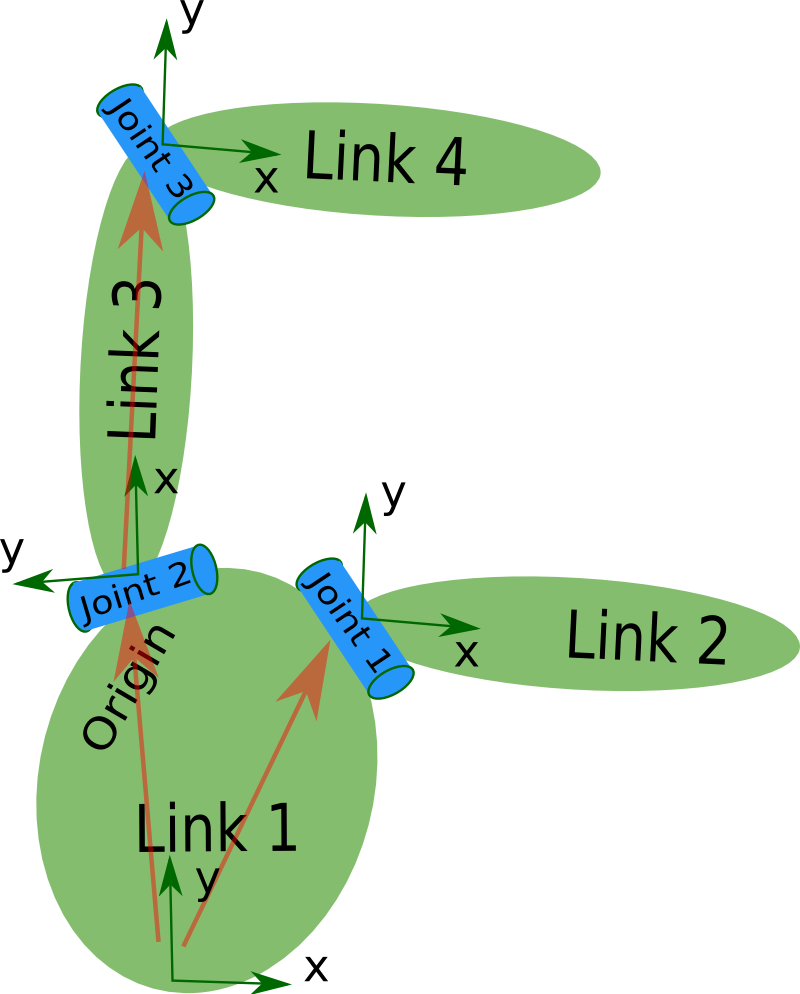
\includegraphics[width=5.5cm]{images/urdf_model.png}
	\caption{Aufbau URDF \cite{ros}}
	\label{Ab:aufbaut-urdf}
\end{figure}

\subsubsection{Link}
\label{chap:link}
Das Link"=Element beschreibt ein einzelnes Glied vom Roboter.
Der Ursprung vom Link ist der gleiche, wie der Ursprung vom Joint.
Folgende Informationen sind als Sub"=Elemente enthalten: 
\begin{itemize}
\item Massenträgheit
\item Geometrie und Material für Aussehen
\item Geometrie für Kollisionsberechnung
\end{itemize}
Für jedes dieser aufgelisteten Sub"=Element muss dessen Ursprung bezüglich des Link"=Ursprungs angegeben werden (dargestellt durch drei schwarze und gekrümmte Pfeile in Abbildung \ref{Ab:aufbaut-link} ).
\begin{figure}[ht!]
	\centering
	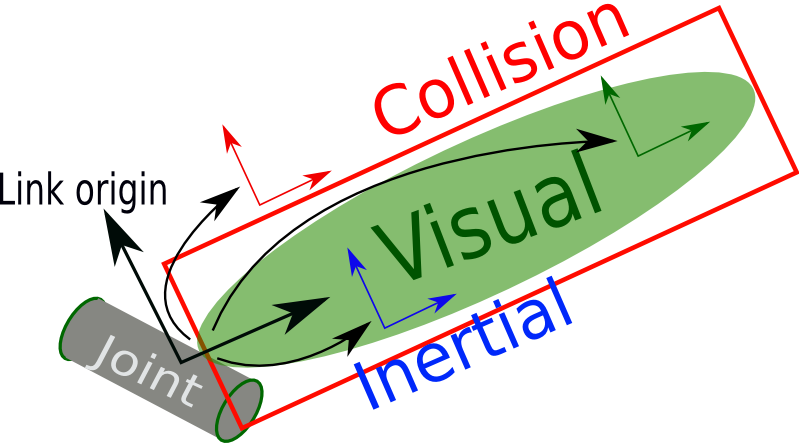
\includegraphics[width=5.5cm]{images/urdf_link.png}
	\caption{Schematische Darstellung Link"=Element \cite{ros}}
	\label{Ab:aufbaut-link}
\end{figure}
%TODO ref listiting motor

\subsubsection{Joint}
\label{chap:joint}
Mit dem Joint"=Element können Gelenke unterschiedlichster Art beschrieben werden.
Folgende Informationen braucht es zur Beschreibung eines Gelenks:
\begin{itemize}
\item Gelenk"=Type
\item Gelenk"=Ursprung (als Transformation gegenüber Ursprung vom Eltern Link)
\item Eltern Link"=Element
\item Kind Link"=Element
\end{itemize}
Die zwei häufigsten Gelenk"=Typ die verwendet werden sind:
\begin{itemize}
\item \textsc{"}kontinuierliche\textsc{"} Typ, freie Rotation um eine Achse (continuous)
\item \textsc{"}fixe\textsc{"} Type, beide Links fest verbunden (fixed)
\end{itemize} 
Die Beziehung dieser Angaben  zueinander ist in Abbildung \ref{Ab:aufbaut-joint} dargestellt.
\begin{figure}[ht!]
	\centering
	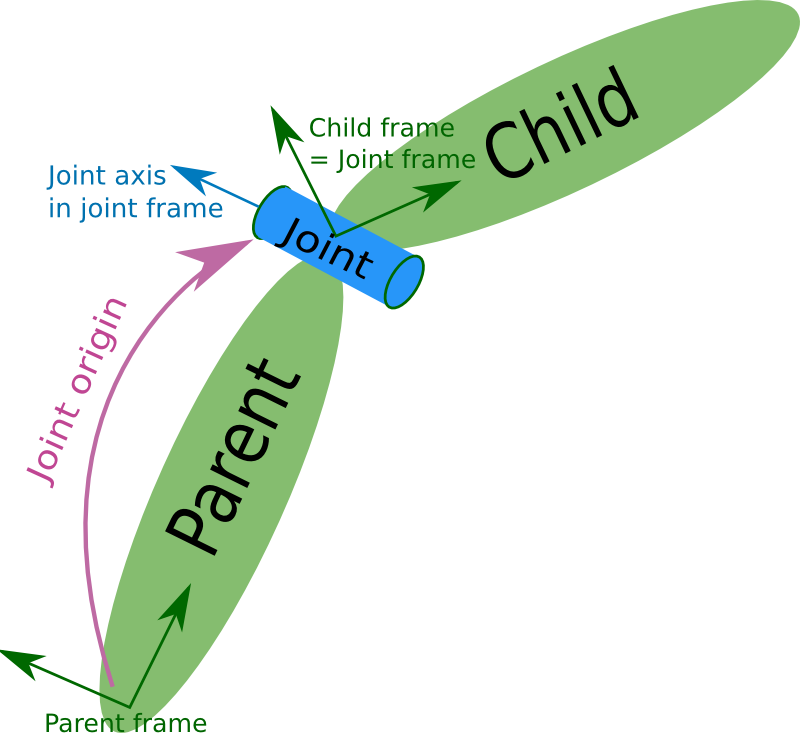
\includegraphics[width=5.5cm]{images/urdf_joint.png}
	\caption{Schematische Darstellung Joint"=Element \cite{ros}}
	\label{Ab:aufbaut-joint}
\end{figure}


%Wie ein Joint"=Element aufgebaut sieht man in der Auflistung xx. %TODO ref listing motor


\section{Transformationen} % Bezugssystem
\label{chap:transformationen}
Eine Transformation beschreibt, wie ein Koordinatensystem relativ zu einem anderen steht.
Koordinatensysteme beschreiben eine Position und Orientierung im Raum, für zum Beispiel ein Glied.
%Die Position und Orientierung eines Körpers im Raum kann mit einem Koordinatensystem beschrieben werde.
Aufbau einer Transformation:
\begin{itemize}
\item Bezeichnung von Eltern"=Koordinatensystem bzw. Eltern"=Glied
\item Bezeichnung von Kind"=Koordinatensystem bzw. Kind"=Glied
\item Translations"=Komponente
\item Rotations"=Komponente
\end{itemize}

Durch die Eltern/Kind Relation bilden die Transformationen eine Baumstruktur.
Das Wurzel"=Element dieses Baumes ist meistens das Welt"=Koordinatensystem.

%In \textit{ROS} werden aber nicht \textsc{"}absolute\textsc{"} Koordinatensysteme verwendet, sondern Transformationen zwischen den Koordinatensystemen.
%Somit sind die Position und Orientierung eines Koordinatensystems immer in Bezug  zu einem  

Zur Veranschaulichung dieser Sachverhalte wird ein Beispiel eines einfachen Roboters mit zwei Gliedern und einem Gelenk gezeigt (zusehen in Abbildung \ref{chap:transformationen}).
Die Transformations"=Baumstruktur (TF-Tree) zu diesem einfachen Roboter ist in Abbildung \ref{Ab:tf-tree} dargestellt.

 %TODO übererbeiten und mit bild tf
% Bild rrbot daneben bild mit tf graph
\begin{figure}[ht!]
\begin{minipage}{0.48\textwidth}
	\centering
	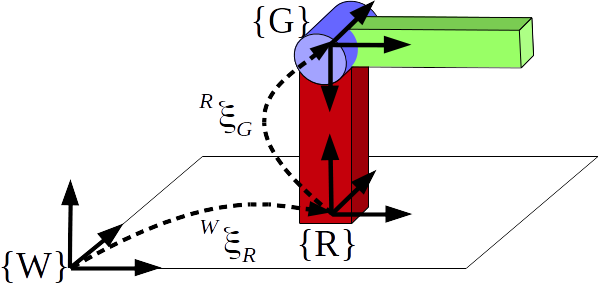
\includegraphics[width=8cm]{images/Transformation.png}
	\caption{Beispiel: Transformation}
	\label{Ab:transformation}
\end{minipage}
\begin{minipage}{0.48\textwidth}
\centering
\begin{tikzpicture}[scale=1,node distance=6.5mm,
	link/.style={rectangle, draw=black, thick, inner sep=7},
	>=latex]
 	
 \node[link] (world) {world}; 
 \node[link, above=of world] (linkR) {link\_R};
 \node[link, above=of linkR] (linkG) {link\_G};
 
 \path[->, thick]
 	(world) edge (linkR)
 	(linkR) edge (linkG);
 
\end{tikzpicture}
	\caption{Beispiel: TF-Tree}
	\label{Ab:tf-tree}

\end{minipage}
\end{figure}

Man berechnet das Koordinatensystem des grünen Gliedes in Bezug zu der Welt wie folgt:
\begin{equation}
^{W}\xi_{G} = ^{W}\xi_{R} * ^{R}\xi_{G}
\end{equation}
Die Angabe für das Koordinatensystem von Objekt \{B\}, in Bezug zu einem Koordinatensystem \{A\}, ist gleichzeitig auch die Transformation ($^{A}\xi_{B}$) von Koordinatensystem \{A\} zu \{B\}.

\subsection{Umrechnung Gelenkwinkel zu Transformationen}
\label{chap:robot-state-publiseher}
Für die Umrechnung von den Winkelpositionen der Gelenke zu den Koordinaten"=Transformationen gibt es in \textit{ROS} den \textit{robot\_state\_publisher}.
Dieser \textit{ROS}"=Node benötigt die Beschreibung des Roboter"=Modells als \textit{URDF}"=Datei.
Er setzt dann die Gelenkwinkel im Modell ein und rechnet anschliessend die einzelnen Transformationen zwischen den Gelenken aus.
Mit diesen Transformationen kann dann \textit{RViz} die Glieder im Raum so positionieren, dass es den Roboter korrekt darstellen kann.

%Der \textit{robot\_state\_publisher} berechnet für jedes Gelenk die Transformationen und gibt sie aus.
%Als Eingabe braucht er zum eine die System"=Beschreibung als \textit{URDF}"=Datei und zum anderen laufend die Winkel"=Positionen zu jedem Gelenk.


%aus den Informationen über den Zustand eines Systems die Transformation 


% oder mehr so was wie: Koordinatensystem, Roboter Zustand
% Transformation 
%joint state publisher erklären für was
%robot state publisher

% erklären wie tf erzeugen tf = Transform, coordinate frame data
%verweis rviz braucht tf daten

